\section{HST Central Light, Revised Uncertainty and Unused Catalogue Targets}
\label{sec:observed-revision}
The first experiment is retained as an exposed development result.
We now address its two concrete failures: overly restrictive brightness
uncertainty and an additional central-image prediction that had not been
tested against pixels. HST data constrain the revised source; a separate
Las Cumbres Observatory (LCO) exposure set tests its subsequent predictions.
Neither reuse of the first targets nor the HST-conditioned profile is
counted as a new independent validation.

\subsection{The original central-image prediction in HST pixels}
We apply the original conventional $0.06320$ and conditional R1 $0.06313$
central/A macro-flux predictions to public
HST ACS/WFC F814W data (proposal 9744, 1445 s, 2003 August 18) and WFC3/IR
F160W data (proposal 12889, 9939.59 s, 2012 October 28). Exact science,
weight and context cutouts and full-product provenance are retained.
Three field-star PSFs and an image-A empirical PSF probe template
dependence. The four outer quasar images determine translation and
rotation; the central template also receives independent freedom of
$\pm50$ mas in each coordinate. The weight maps in these products are
exposure-like, rather than inverse variance; drizzle correlations require
separate attention~\cite{STScIDrizzle}. Blank-sky scatter, relative exposure and
source Poisson noise define the adopted marginal variance.
The nominal bound also permits a 5\% lower image-A flux normalization.

A deliberately flexible bound allows arbitrary nonnegative galaxy,
host and unresolved nuclear light at every pixel. With
$d_p=fP_p+B_p+\epsilon_p$, $P_p\geq0$ and $B_p\geq0$, a fixed-template
Gaussian marginal-error union bound gives
\begin{equation}
 f\leq\min_{p\in\mathcal S}
 \frac{d_p+\Phi_{\rm N}^{-1}(1-0.05/|\mathcal S|)\sigma_p}{P_p},
 \qquad \mathcal S=\{p:P_p>0.03\max P\}.
 \label{eq:hst-positive-bound}
\end{equation}
Here $\Phi_{\rm N}$ is the standard-normal CDF. Pixel independence is
unnecessary. The 95\% interpretation is conditional on the adopted PSF,
sky subtraction and marginal-error model. Maximization over the finite
PSF set and continuous centroid freedom is numerical, not a certified
global or arbitrary-PSF coverage statement.

The F814W numerical envelope is $0.02935$ of A, conservatively rounded
up to $0.030$. Multiplying every marginal noise scale by five and lowering
the A normalization by 20\% increases it to $0.04124$, conservatively
rounded to $0.042$. Both are below the original $0.06320$ prediction.
The noise/normalization stress test is a sensitivity control, not an
independent calibration of 95\% coverage.
F160W gives $0.554$ and is inconclusive. Positive smooth galaxy profiles,
including a free compact cusp and nuclear point, give the same direction
of tension; their residual sums are descriptive, not detection
significances. Figure~\ref{fig:hst-central} shows the pixel application.
This tests the achromatic, unattenuated macro ratio. Differential
extinction, microlensing or intrinsic variability across the central-image
delay are not inferred here; retaining the old profile with such effects
requires a separate physical flux prescription.

\begin{figure}[htbp]
 \centering
 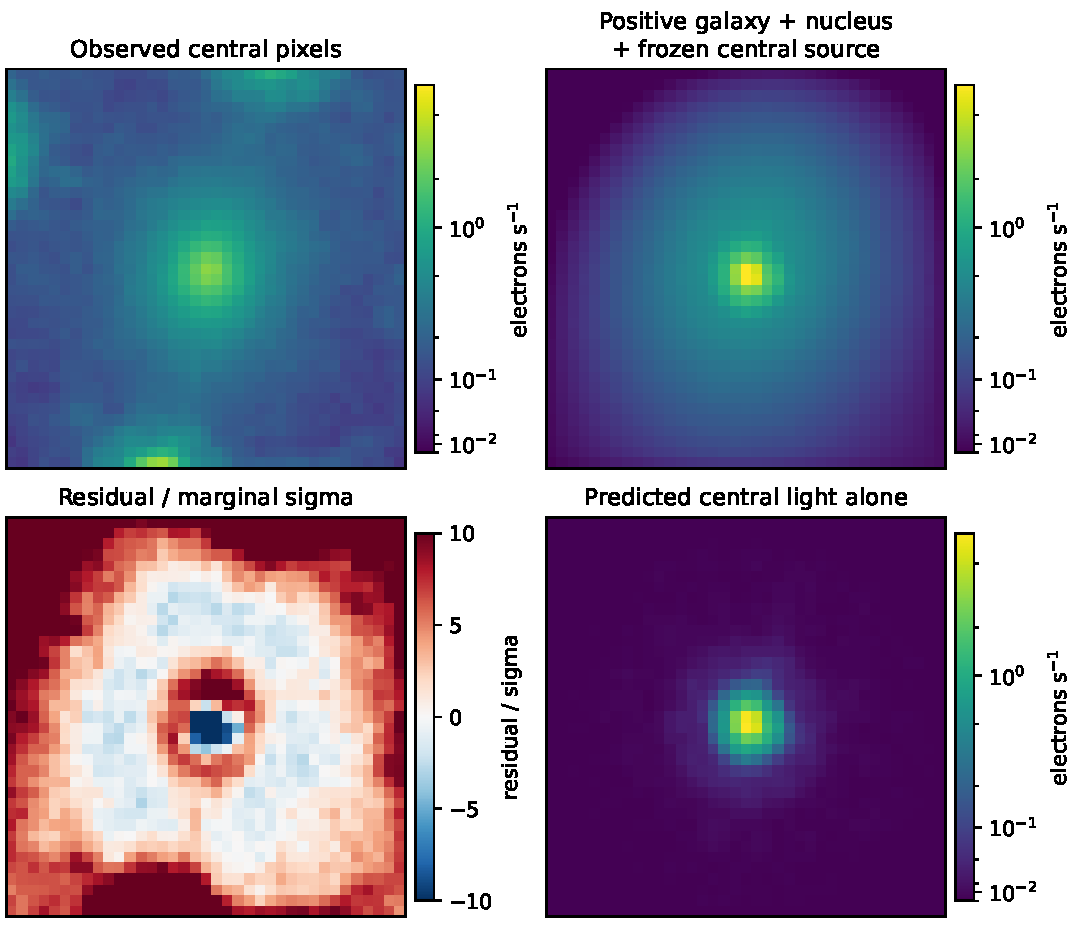
\includegraphics[width=0.96\textwidth]{figures/he0435_hst_central_pixel_test.pdf}
 \caption{Actual ACS F814W pixels and the original central-image application.
 Upper left: measured central pixels; upper right: a fitted positive
 galaxy/cusp/nuclear-light model plus the frozen central source. Lower
 left: residual divided by the adopted marginal noise (colour range
 clipped at $\pm10$); lower right: predicted central light alone.
 Intensity colour bars are in electrons per second.
 The nonnegative-pixel test permits arbitrary positive contaminating
 galaxy/host/nuclear light. Its F814W conditional tension motivates the
 source revision. The separate F160W application does not exclude this
 prediction. HST data are development information in the revised model.}
 \label{fig:hst-central}
\end{figure}

\subsection{A revised source and classical brightness uncertainty}
We retain a regular positive local source by adding a compact Plummer
component to the outer body:
\begin{equation}
 \rho(r)=\sum_{j=\mathrm{o,n}}
 \frac{3M_ja_j^2}{4\pi(r^2+a_j^2)^{5/2}},\qquad
 M(<r)=\sum_{j=\mathrm{o,n}}
 \frac{M_jr^3}{(r^2+a_j^2)^{3/2}}.
 \label{eq:revision-source}
\end{equation}
The compact scale is prescribed as $a_{\rm n}=0.03$ kpc and its candidate
masses are $0,10^8,10^{8.5},10^9,10^{9.5}M_\odot$.
This is a regular unresolved matter surrogate, not a black-hole mass
measurement. The original R1 nonlinear equation consumes the \emph{total}
$M(<r)$ once; independently solved component scalars cannot be added.
The original regular branch, metric Gauss equation, optical projection,
rear screen and nine nuisance parameters are otherwise retained.

For each conventional candidate, original astrometry and the exact
development brightness likelihood determine the optical parameters.
HST assesses the \emph{sum} of every additional-image PSF, including
unresolved multiple nuclear images. Among HST-admissible candidates the
development objective selects one common compact mass for both models.
The R1 model then refits its nuisance parameters using the same data.
Candidate traces and the separate fixed-body R1 activation remain visible;
this discrete profile selection does not define a posterior mass interval.

The revised classical brightness law is
\begin{align}
 u&=t+\delta_k-d_i,\nonumber\\
 m_{ik}(t)&=m_0+b_{ik}+q(u)+e_i(u)
             +a_i\frac{u-t_0}{Y}+w_i(u)+\epsilon_{ik},
 \qquad Y=365.25\ {\rm day}.
 \label{eq:revision-brightness}
\end{align}
The source $q$ and individual extrinsic processes $e_i$ are independent
stationary OUs. Gaussian slopes have standard deviation
$0.03$ mag yr$^{-1}$, and independent Brownian increments have covariance
$D_i^2\min(u-t_0,v-t_0)/Y$. Proper per-image/instrument offsets have
30-mag prior width, accommodating the distinct relative and apparent
magnitude zeros without a target-derived offset. Quoted marginal errors
plus per-image jitter supply measurement variance. Slopes and Brownian
increments propagate increasing uncertainty beyond the last observation;
all latent processes are conditioned jointly by the original state-space
likelihood. Brownian increments start at zero at $t_0=52832$ in native day
units, the floor of the earliest development epoch minus 31 days; this
precedes every allowed shifted observation. None is a BHSM statistical-state contraction.

All 1002 old epochs and 25 pre-2019 LCO R epochs are development data.
Three 500-day and three 2000-day rolling-origin windows recalibrate
per-image uncertainty. The longer windows were added before numerical
target inspection because known timestamps extend about five years past
calibration. Overlapping development windows are not independent
replications. The unchanged higher empirical 97.5th-percentile rule gives
primary A/B/C/D scale factors $(1,3.61321,1,1)$ and all-image forecast
factors $(1.61012,1.90726,1.87754,1.92479)$. In particular, short-window
calibration alone misses longer-horizon B undercoverage.

A frozen 72-component finite nuisance ensemble propagates retained
parameter variation and catalogue epoch-origin offsets $(-0.5,0,+0.5)$ day. It is
constructed from two short correlated chains and three development-only
epoch-origin reweightings, not 72 independent posterior draws. Between-chain
$\widehat R$ reaches $5.19$ for weak extrinsic/Brownian decomposition
and about $2.16$ for source amplitude/time scale. Posterior convergence
is not established; this is a specified empirical predictive algorithm,
not a complete marginalized physical posterior. Fixing macro delays
transports the ensemble with development likelihood-ratio weights.
Driver conditioning subsequently updates weights and latent states only.
The per-image affine calibration includes its joint-density Jacobian.
We therefore assess both coverage and the cost in interval width and
proper score on the new observations.

\subsection{Unused LCO catalogue targets}
The separate CTIO 1-m LCO monitoring~\cite{Sorgenfrei2025} supplies
54 R epochs from 2019 through 2024 beyond every consumed COSMOGRAIL
epoch. Its earlier 25 R epochs calibrate the instrument; all 80 V epochs
remain unscored. Before opening R target values we fixed the split,
model, calibration and source hashes and committed their predictive
artifact. The primary application allows the 54 C magnitudes as a batch
driver and withholds the 162 A/B/D magnitudes. C was selected using
consumed first-experiment behavior. The secondary forecast withholds all
216 magnitudes and overlaps the primary test.

These numerical catalogue targets were unused by our model fitting and
selection, with explicit limitations. The published LCO reduction
uses a common difference-imaging reference mostly assembled from 2022;
the exact reference-exposure list and full photometric covariance are
unavailable. Common offsets capture static calibration uncertainty,
but a full reference-noise likelihood is not identified by the released
marginal errors. Numerical target values were unused; photon-disjoint calibration and full
reference-noise independence are not established. The experiment is a
retrospective catalogue-withholding test, not an independently blinded
reduction or prospective forecast.
Source identification also exposed qualitative published microlensing
findings; numerical catalogue targets and plots were not inspected
before freezing. Complete analyst blinding is not claimed.

\subsection{Revised source and frozen diagnostics on unused catalogue values}
\label{sec:he0435-revised-results}
The development selection retains candidate 1 with a regular compact matter component of \(1.000\times10^{8}\)\,$M_\odot$ and scale 0.03\,kpc.
The conventional and conditional R1 applications have 5 and 5 verified stationary images, respectively; all additional images enter the summed central-light constraint.
The nearly degenerate development objectives do not measure a nuclear mass. The selected positive component is a conditional matter surrogate, not an inferred black hole or a solved stellar equation of state.

The original scalar and metric equations are applied to the total enclosed matter once:
\[ Cx^2p-\frac{4}{\widehat\lambda}xp^2=-\widehat b\,m(x),\qquad 2x^2\frac{d\Phi}{dx}+\widehat b x^2p=2m(x). \]
Here $x=rH_0$, $m(x)=GM(<r)H_0$, $\widehat b=b_T/M_{\rm Pl}$, $p=\pi_T^{\prime}/(M_{\rm Pl}H_0)$ and $c=1$, with the previously fixed $\widehat\lambda=\lambda/(M_{\rm Pl}H_0^2)$.
At $r=0.03$\,kpc, the computed section has $\widehat\rho=\rho/(M_{\rm Pl}^2H_0^2)$ equal to \(3.734\times10^{9}\), reduced source $\widehat J_{\rm eff}=J_{\rm eff}/(M_{\rm Pl}H_0^2)=-\widehat b\widehat\rho/2$ equal to \(-1.712\times10^{8}\), and $p$ equal to \(-3.599\times10^{-5}\).
The scalar integrated left side and source are \(-3.495\times10^{-17}\) and \(-3.495\times10^{-17}\), while the metric Gauss left side and source are \(7.623\times10^{-16}\) and \(7.623\times10^{-16}\).
Across the evaluated sections the maximum relative scalar and Gauss residuals are \(3.419\times10^{-16}\) and \(2.168\times10^{-16}\).
Activating R1 on the fixed conventional body, source, maps and clock gives B/C/D-minus-A delay offsets $(20.60284,1.00422,31.21607)$\,s and a maximum coordinate image displacement \(2.075\times10^{1}\)\,$\mu$as. Separately refitted model predictions below need not retain those fixed-reference offsets.

The compact-source model's LCO test opens 162 previously unused A/B/D measurements, conditional on 54 allowed C measurements from the same later LCO epochs. The no-driver secondary forecast opens all 216 measurements. No brightness, delay, offset, calibration or source parameter is refitted to these target values. These scores belong to this frozen geometry, preceding the explicit G1 revision below.
Table~\ref{tab:he0435-revised-primary} reports the normalized joint conditional density and marginal predictive diagnostics. The joint log density is a density in the declared magnitude units; epochs are correlated, and its value is not a chi-square significance or an independent-event count.
\begin{table}[t]
\caption{Frozen compact-source models on unused LCO R A/B/D observations, with image C as the allowed driver. Coverage is the empirical fraction within marginal 95\% mixture intervals; width and the proper 95\% interval score are in magnitudes. Larger joint log density and smaller interval score are preferred.}\label{tab:he0435-revised-primary}
\centering\footnotesize
\begin{tabular}{lrrrrr}\toprule
Model & Joint $\log p$ & RMSE & \shortstack{95\%\\coverage} & Width & \shortstack{95\%\\interval score}\\\midrule
Empirical delay ensemble & 292.467 & 0.0780 & 98.77 & 0.6566 & 0.6640\\
Conventional macro & 291.071 & 0.0772 & 98.77 & 0.6699 & 0.6779\\
Conditional R1 macro & 291.071 & 0.0772 & 98.77 & 0.6699 & 0.6779\\
Fixed-body R1 activation & 291.071 & 0.0772 & 98.77 & 0.6699 & 0.6779\\
Zero-delay control & 289.016 & 0.0795 & 98.77 & 0.6245 & 0.6334\\
\bottomrule\end{tabular}
\end{table}

The old undercoverage is not reproduced in this unused-catalogue batch, but the revised uncertainty is conservative rather than sharply calibrated: nominal 68.27\% intervals contain 94.44\% of primary targets, and image B has mean 95\% width 1.3014\,mag. The no-driver secondary forecast retains mean signed residual +0.1761\,mag. Moreover, the zero-delay control has mean 95\% interval score 0.6334\,mag, compared with 0.6779\,mag for conventional, while conventional has the larger joint log density. Coverage, width, bias and the different proper scores must therefore be considered together; no uniformly superior model or precise delay recovery is established by this batch.
The conventional intervals contain 160 of 162 primary targets (98.77\%). The conditional R1-minus-conventional joint log-score difference is \(-3.460\times10^{-5}\); this is a finite-model predictive comparison, not a Bayes factor from a completed physical-state posterior.
The fixed-body R1 activation has a primary log-score difference of \(1.507\times10^{-4}\) relative to conventional, with the same optical nuisance parameters. It isolates the original scalar response; the separately refitted R1 comparison also includes development nuisance and optimizer movement and cannot be attributed entirely to that activation.
The matched conventional effective-mass representation has the same retained optical transfer as conditional R1 and therefore the same score by construction; it is not an independent confirmation.
\begin{table}[t]
\caption{Image-resolved primary diagnostics. Each image contributes 54 unused observations. These are correlated marginal diagnostics, not 54 independent coverage trials.}\label{tab:he0435-revised-images}
\centering\small\begin{tabular}{lrrr|rrr}\toprule
&\multicolumn{3}{c}{Conventional}&\multicolumn{3}{c}{Conditional R1}\\
Image & RMSE & Coverage (\%) & Width & RMSE & Coverage (\%) & Width\\\midrule
A & 0.0489 & 96.30 & 0.3667 & 0.0489 & 96.30 & 0.3667\\
B & 0.1192 & 100.00 & 1.3014 & 0.1192 & 100.00 & 1.3014\\
D & 0.0361 & 100.00 & 0.3417 & 0.0361 & 100.00 & 0.3417\\
\bottomrule\end{tabular}
\end{table}

Without the C driver, the conventional all-image forecast has joint log density 390.118, RMSE 0.2170\,mag, 95\% coverage 100.00\%, mean interval width 1.2534\,mag and mean interval score 1.2534\,mag. The secondary R1-minus-conventional log-score difference is \(2.497\times10^{-6}\). Primary and secondary targets overlap and cannot be counted as separate confirmations.
\begin{figure}[t]
\centering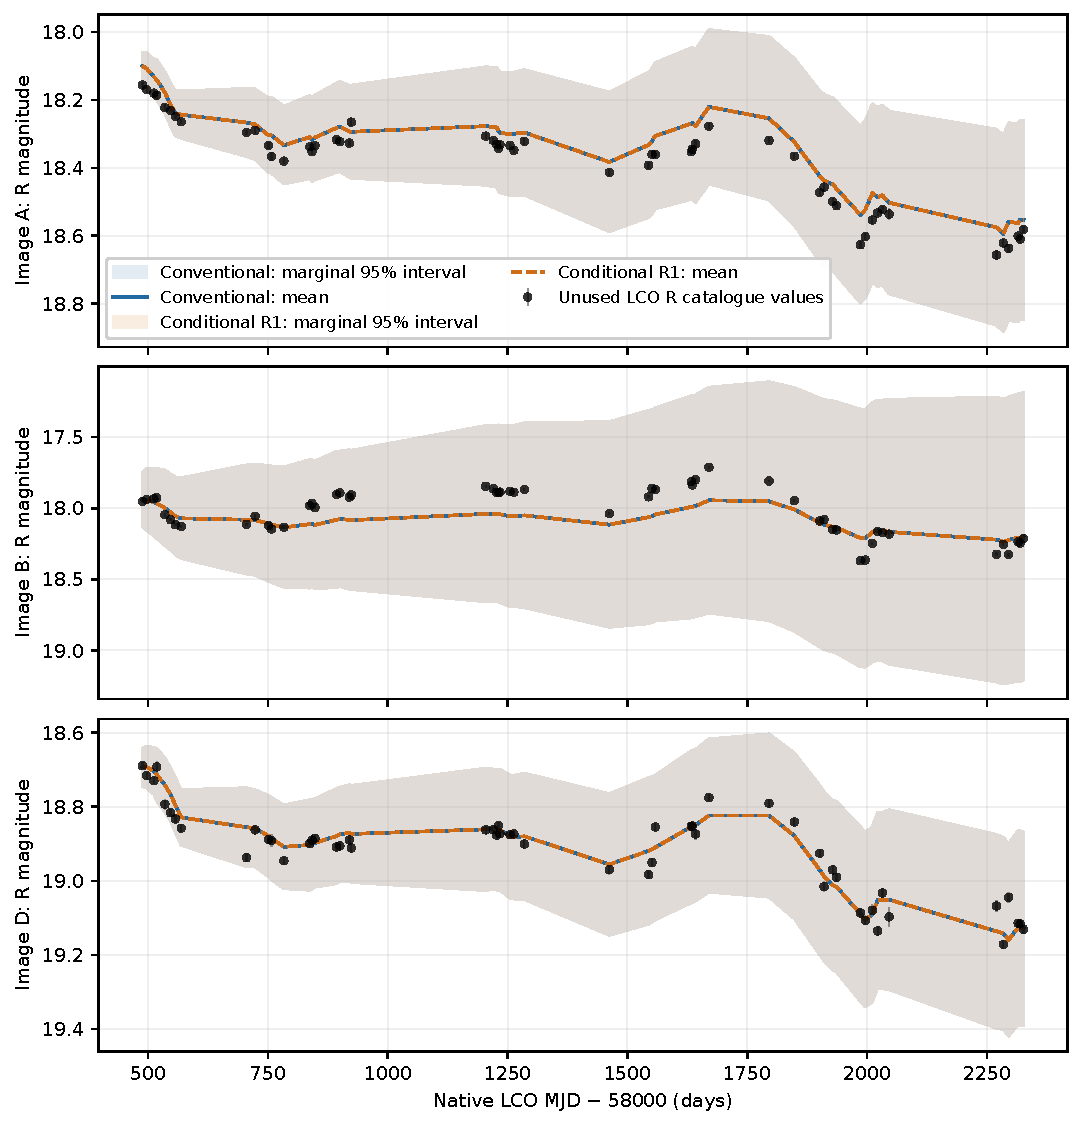
\includegraphics[width=\textwidth]{figures/he0435_revision_unused_prediction.pdf}
\caption{Unused LCO R observations and the frozen C-driven conventional and conditional R1 predictions. Shading shows marginal 95\% mixture intervals, including the development-only image calibration. The curves and bands can nearly coincide. Straight segments join predictions only at observed epochs and are not an additional fitted variability curve.}\label{fig:he0435-revised-unused}
\end{figure}

The experiment tests a fixed, calibrated finite nuisance ensemble. Its short chains have maximum basic $\widehat R=5.19$, so the mixture is not a demonstrated converged posterior and supplies no complete physical-state marginalization. These LCO catalogue values were unused in model selection and arise from a separate monitoring campaign. Their retrospective difference-imaging reference includes 2022 data, however, so photon-disjoint calibration and validation are not established. Common reduction errors and prior qualitative publication awareness limit blinding. The central-image HST result is conditional on the empirical PSFs, adopted marginal noise and macro-to-observed flux relation. These qualifications, and any remaining undercoverage in the actual test, remain part of the result. Neither the statistical ensemble nor a close conventional/R1 score establishes a unique envelope state or a BHSM detection; the physical guard remains $2\times10^{-10}$ and no physical admission is asserted.

\subsection{A separate unused Gaia astrometric test}
\label{sec:he0435-gaia}
The LCO common-reference limitation motivates a second type of observation:
the four image positions in Gaia DR3~\cite{GaiaDR3}. We declare this
additional test after the LCO result is known, while retaining exactly the
already-frozen conventional and R1 physical predictions. A count-only
catalogue query establishes four entries in the lens field. Numerical
positions, errors and quality rows remain unopened until a separate
prediction/protocol commit. No mass, screen, source, angle, plate scale or
rotation is fitted against Gaia.

In a common small-angle ICRS tangent frame the three relative observables
are $z_i=((\alpha_i-\alpha_A)\cos\delta_A,\delta_i-\delta_A)$,
$i=B,C,D$, with degree-to-arcsecond conversion. All 24 source assignments
are compared with the fixed conventional relative pattern; the same
assignment is used for R1 and its runner-up gap is retained. For each Gaia
source, the published RA tangent-plane error
$\sigma_{\alpha*}=\sigma_\alpha\cos\delta$, declination error and their
correlation define $C_i$. The RA error receives no second cosine.
The full six-coordinate formal covariance is
\begin{equation}
 [C_{\rm rel}]_{ij}=\delta_{ij}C_i+C_A,
 \qquad C_s=C_{\rm rel}+s^2I_6,
 \quad s=0,2,5\ {\rm mas}.
 \label{eq:gaia-covariance}
\end{equation}
The added floors apply per relative coordinate after differencing; they
are prespecified sensitivity controls, not fitted noise or a derived macro
posterior. The Gaussian density and quadratic residual use $C_s$, including
its determinant and common-A off-diagonal blocks. Between-source catalogue
covariances are unpublished, so source-error independence remains a
conditional approximation. All four sources are retained irrespective of
their quality diagnostics; missing mandatory errors cannot be replaced
silently with zero correlation.

Gaia collected different photons in 2014--2017, whereas the fitted NIC2
point astrometry was published in 2011. However, the reprocessed HST central
mosaics use a Gaia-EDR3 field frame. Their pixel test uses relative
registration, but independence of every field calibration is not certified.
Close-image blending, chromatic photocentres and fixed macro parameters
further limit a catalogue-only Gaussian interpretation. This test assesses
the previously unused numerical quasar geometry; it is not a complete
Einstein-ring reconstruction or a BHSM state measurement.

The Gaia prediction freeze was committed before the numerical query.
The unique closest A/B/C/D assignment has squared residual
$6.3594\times10^{-5}$ arcsec$^2$; the runner-up is $4.6197$ arcsec$^2$.
No continuous frame parameter is fitted. The conventional observed-minus-
predicted east/north residuals are $(0.623,1.701)$ mas for B,
$(1.915,-5.026)$ mas for C and $(-5.572,0.580)$ mas for D.
Their coordinate RMS is $3.25560$ mas, versus $3.25557$ mas for R1.
Table~\ref{tab:gaia-frozen} reports every prespecified covariance control.

\begin{table}[htbp]
 \centering
 \caption{Previously unused Gaia DR3 relative astrometry, with all physical
 predictions fixed before the query. $Q=r^TC_s^{-1}r$ uses six coordinates;
 the log density is normalized in mas$^{-6}$. Added floors are sensitivity
 controls, not fitted errors or a completed macro posterior.}
 \label{tab:gaia-frozen}
 \begin{tabular}{lrrrr}
 \toprule
 Floor (mas) & Conventional $Q$ & R1 $Q$ & Conventional $\log p$ & R1 $\log p$\\
 \midrule
 $0$ & $3465.905$ & $3465.667$ & $-1727.177$ & $-1727.058$\\
 $2$ & $15.7966$ & $15.7963$ & $-17.5910$ & $-17.5908$\\
 $5$ & $2.54112$ & $2.54107$ & $-16.4441$ & $-16.4440$\\
 \bottomrule
 \end{tabular}
\end{table}

Both frozen point predictions fail the catalogue-error-only precision
check. The source RUWE values are $1.00$--$1.11$, none is marked duplicated,
and multi-peak fractions are 0--1\%. B and D nevertheless have odd-window
fractions of 64\% and 69\%, and C has excess-noise significance 2.57;
these diagnostics remain visible without post-target image exclusion.
Adding the declared floors reduces the
formal mismatch, but cannot turn a sensitivity calculation into successful
validation or establish the required physical uncertainty. The R1-minus-
conventional log densities are $0.1191$, $1.53\times10^{-4}$ and
$2.43\times10^{-5}$ for the three controls. A small difference between
inadequate point predictions is not evidence for a BHSM state.
The next physical inference requires justified training/frame/photocentre
and macro-model uncertainty together with richer mass/environment
constraints. These Gaia targets are now consumed; fitting them later
cannot count as another unused-data success.


